\chapter{Dark matter: Beyond the Standard Model}
\label{chap:DM}
%% Restart the numbering to make sure that this is definitely page #1!
\pagenumbering{arabic}

The Standard Model (SM) of particle physics, albeit a successful theory encoding the properties of elementary particles and their interactions, nonetheless has some shortcomings. For one, cosmological and astrophysical observations supply compelling evidence~\cite{Bertone:2004pz, Feng:2010gw, Porter:2011nv} for the existence of dark matter (DM), a piece of the astro-particle physics puzzle that does not fit together with the SM. In Sec.~\ref{sec:DMintro}, evidence of the existence of DM and motivations for its search are briefly detailed, while in Sec.~\ref{sec:DMsearches} the three main modes of DM detection are outlined, with a particular emphasis on particle colliders. An outline of the SM is presented in Sec.~\ref{sec:SM} and its connection with DM is described in Sec.~\ref{sec:BSM}, with a focus on beyond the Standard Model (BSM) simplified models of DM currently being probed at general-purpose detectors at the Large Hadron Collider (LHC) in Geneva, Switzerland.

\section{Introduction to dark matter}
\label{sec:DMintro}

Observations at all scales, from smaller dwarf galaxies to large cosmological scales point to the existence of more matter than can be reconciled with the amount of visible matter in our universe. The existence of additional non-luminous matter and its dominance in amount compared to luminous matter, was first postulated by Swiss physicist Fritz Zwicky in 1933 during his studies of the Coma cluster. Zwicky's observations pointed to the necessity for approximately 400 times~\cite{2009GReGr} the mass density as observed from the luminous matter from the cluster to ensure the gravitational bounding of nebulae within Coma. It is worth noting that Zwicky's calculations made extensive use of Hubble's constant at the time, H$_0$ = 558 km/s/Mpc, and if rescaled by the modern value of H$_0 = 67.27 \pm 0.66$ km/s/Mpc~\cite{Ade:2015xua} Zwicky's results point to approximately a mass density 10 times larger than observed~\cite{Bertone:2016nfn}. The period around the 1950's and 1960's marks a time when various astronomical explanations for the missing mass in galaxy clusters began to be ruled out, such as the hypothesis that dark matter consists of hot intracluster gas. Ref.~\cite{MEEKINS1971} presents evidence that the amount of gas required for gravitational binding is $98\%$ larger than that observed from X-ray emission spectra. During the 1970's the first explicit statements began to emerge regarding the need of the missing mass to be concentrated in the outer parts of galaxies based on spectroscopic and radio astronomy observations of the galactic rotation velocity curves. Namely, Kent Ford and Vera Rubin published results from observations of the Andromeda galaxy which extended the observational reach out to 110 minutes of arc away from the center of M31, revealing a flat dependence of \textit{v}, the galactic rotation velocity, as a function of the radius \textit{r} beyond the visible galactic disk as shown in~\FigureRef{fig:rubin}. By the onset of the 1980's the majority of the astrophysical community was convinced that a substantial amount of DM exists in the universe based on the observational evidence of mass-to-light ratios of galaxies and galactic rotation curves.

\begin{figure}
  \centering
  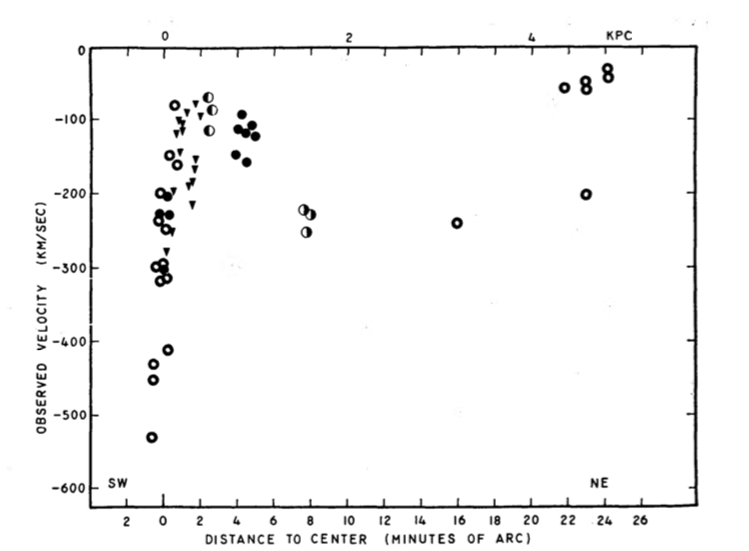
\includegraphics[width=\textwidth]{figs/RubinFordVel}
  \caption{The velocities of emission regions from M31 as a function of distance to the center of the galaxy measured in minutes of arc along the NE major axis as reported by Rubin and Ford in Ref.~\cite{Rubin:1970zza}.}
\label{fig:rubin}
\end{figure}

Studies of the large scale structure of the universe have provided clues as to the nature of dark matter. Just as on the small scale, ordinary visible matter consists of protons, electrons, neutrons, or groups of atoms held together by the electromagnetic force, analogously groups of matter peaks containing stars were bound together by the gravitational force provided sufficiently massive in order to form stellar clusters. These groups were in turn merged with gas and the postulated DM to form galaxies and the galaxies were bound together to form clusters, and superclusters. This standard theory of cosmic structure formation is often referred to as the ``bottom-up'' approach, and essentially posits that the current structure of the Universe is a result of the gravitational amplification of tiny matter fluctuations that were generated during the very early epochs of the Universe~\cite{Allen:2002eu}. The evidence from the 20th century for the existence of non-luminous matter has been further supplemented with data from weak~\cite{Refregier:2003ct} and strong~\cite{Tyson:1998vp} gravitational lensing by large scale structures. The distortion of the appearances of distant objects or the duplication of the apparent image is caused by the bending of the light these objects emit by the gravitational force of the large scale structures in between the observer and the object. The data from a survey of the Bullet cluster as observed by the Chandra~\cite{Markevitch:2005vi} experiment best illustrates how the distribution of the hot gas and stars originating from the collision of two galaxies and comprising the baryonic matter are bound together by a much greater contribution of non-luminous matter as seen in~\FigureRef{fig:bulletcluster}. The calculation of the approximate contribution of visible matter was performed using data from gravitational lensing.

\begin{figure}
  \centering
  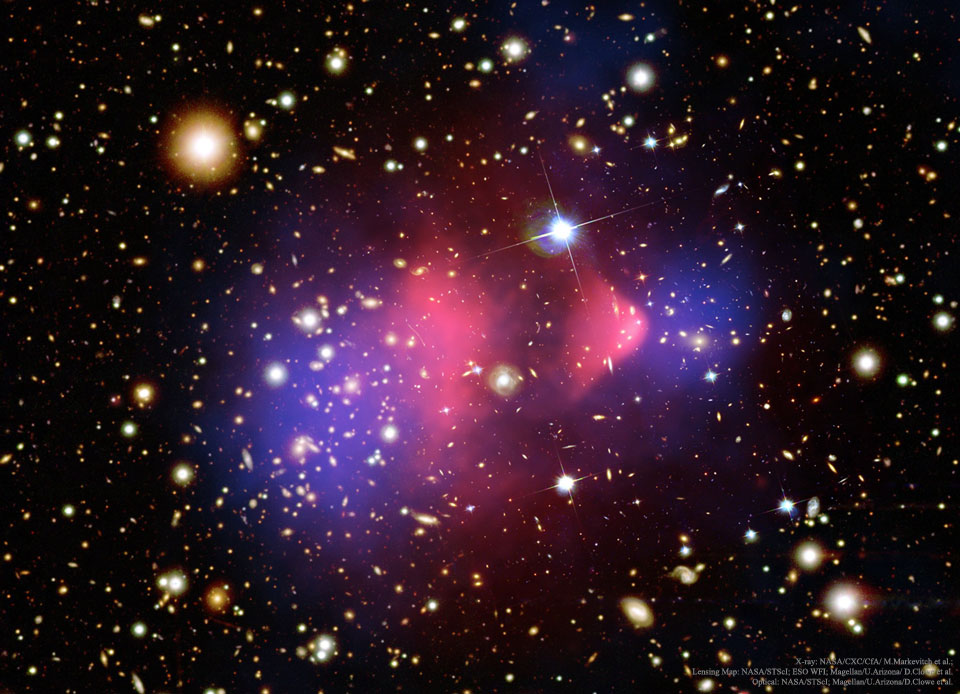
\includegraphics[width=0.8\textwidth]{figs/bulletcluster_comp_960.jpg}
  \caption{A composite image from the Hubble, Chandra, and Magellan telesopes of the 1E 0657-558 cluster of galaxies (Bullet cluster) depicting the X-rays emitted by the baryonic matter as a diffuse red gas, while the approximate location of the DM surrounding the visible matter is represented in a blue hue.}
\label{fig:bulletcluster}
\end{figure}

The aforementioned experiments and measurements buttress the necessity for the existence of DM, however the first attempts to precisely quantify the amount of DM in the Universe began with discovery and subsequent analyses of the cosmic microwave background (CMB) by Peebles, Wilkinson, Dicke, and Roll~\cite{Dicke1965}. In brief, the CMB is the relic radiation energy content from beyond our galaxy, emitted shortly before the period of recombination~\cite{Seager:1999km} which occured approximately 380 000 years after the Big Bang. At this stage, photons began to decouple from the baryonic matter and over time have been redshifted to the microwave frequency range as a result of the expansion of the Universe over the past 13.81 billion years. Although the dominant contributions of the CMB are homogeneous and isotropic wherein the CMB temperature is almost uniformly $T\simeq2.72\:\mathrm{K}$, slight temperature fluctuations of $\mathcal{O}(10^{-5})$ have been observed which are indicative of the state of the early Universe and the relative abundance of visible and dark matter during this period. As gravity acted on the photon-baryon plasma, the fluid pressure increased giving way to its expansion. This cycle was repeated once the pressure decreased as a result of the expansion, and gravity once more won over causing a fluid compression, hence the photons emitted during compression stages were of varying energies. More specifically, the period of photon decoupling leading to these relic temperature variations, known as the CMB anisotropy, can be interpreted as a power spectrum in terms of multipole orders, $\ell$. The effects produced by the acoustic oscillations of the photon-baryon plasma just prior to the emission of the CMB are captured in this spectrum. Since both types of matter contribute to the temperature oscillations via gravitational effects, the power spectrum shown in~\FigureRef{fig:CMB} contains information about the relative content of both visible and dark matter. The parametrization of the temperature anisotropies is in terms of spherical harmonics contained in the two-dimensional function, $T(\theta,\phi)$ projected over the entire visible sky defined as,

\begin{equation}
  T(\theta,\phi) = \sum^{\infty}_{\ell=0}\sum^{\ell}_{m=-\ell}a_{\ell m}Y_{\ell m}(\theta,\phi),
\end{equation}

where $\theta$ and $\phi$ are angular coordinates, $\ell$ is the multipole order, and $a_{\ell m}$ are the multipole moments. Following the theory of temperature fluctuations, the distributions of the coefficients $a_{\ell m}$ are approximately Gaussian centered about zero with a variance defined as $C_{\ell} \equiv <|a_{\ell m}|^{2}>$, where there are only $2\ell+1$ values of $m$ for each $\ell$, hence

\begin{equation}
  C_{\ell} \equiv <|a_{\ell m}|^{2}> \equiv \frac{1}{2\ell+1}\sum^{+\ell}_{m=-\ell}|a_{\ell m}|^2.
\end{equation}

The power spectrum, $C_{\ell}$ is expressed as $\ell(\ell+1)C_{\ell}/2\pi$ in~\FigureRef{fig:CMB}, and fit to the Planck data provides the abundances of baryonic and dark matter. The location of the first peak is related to the flat geometry of the Universe and requires that the total energy-matter density ratio, $\Omega_\mathrm{total}=1$. The resolution of this peak is connected to the expansion of the Universe which is driven by the repulsive force of dark energy~\cite{Spergel:2006hy}. The angular resolution of the second peak, at $\ell_{2}\simeq500$, provides the amount of ordinary matter that exists in the Universe, and correspondingly, the difference between the third peak, at $\ell_{3}\simeq700$, and the second peak provides the density of the dark matter in the early Universe. The extracted total densities of baryonic and dark matter are respectively,

\begin{equation}
  \Omega_{\mathrm{b}}h^2 = 0.02222 \pm 0.00023,\:\:\Omega_{\mathrm{DM}}h^2 = 0.1186 \pm 0.0020,
\end{equation}

where $h = H_{0}/100$ is the reduced Hubble's constant. The relic abundances tranlsate to $24\%$ and $4.8\%$ of the total matter in the Universe as being dark and baryonic, respectively, while the rest consists of dark energy~\cite{Agashe:2014kda}.

\begin{figure}
  \centering
  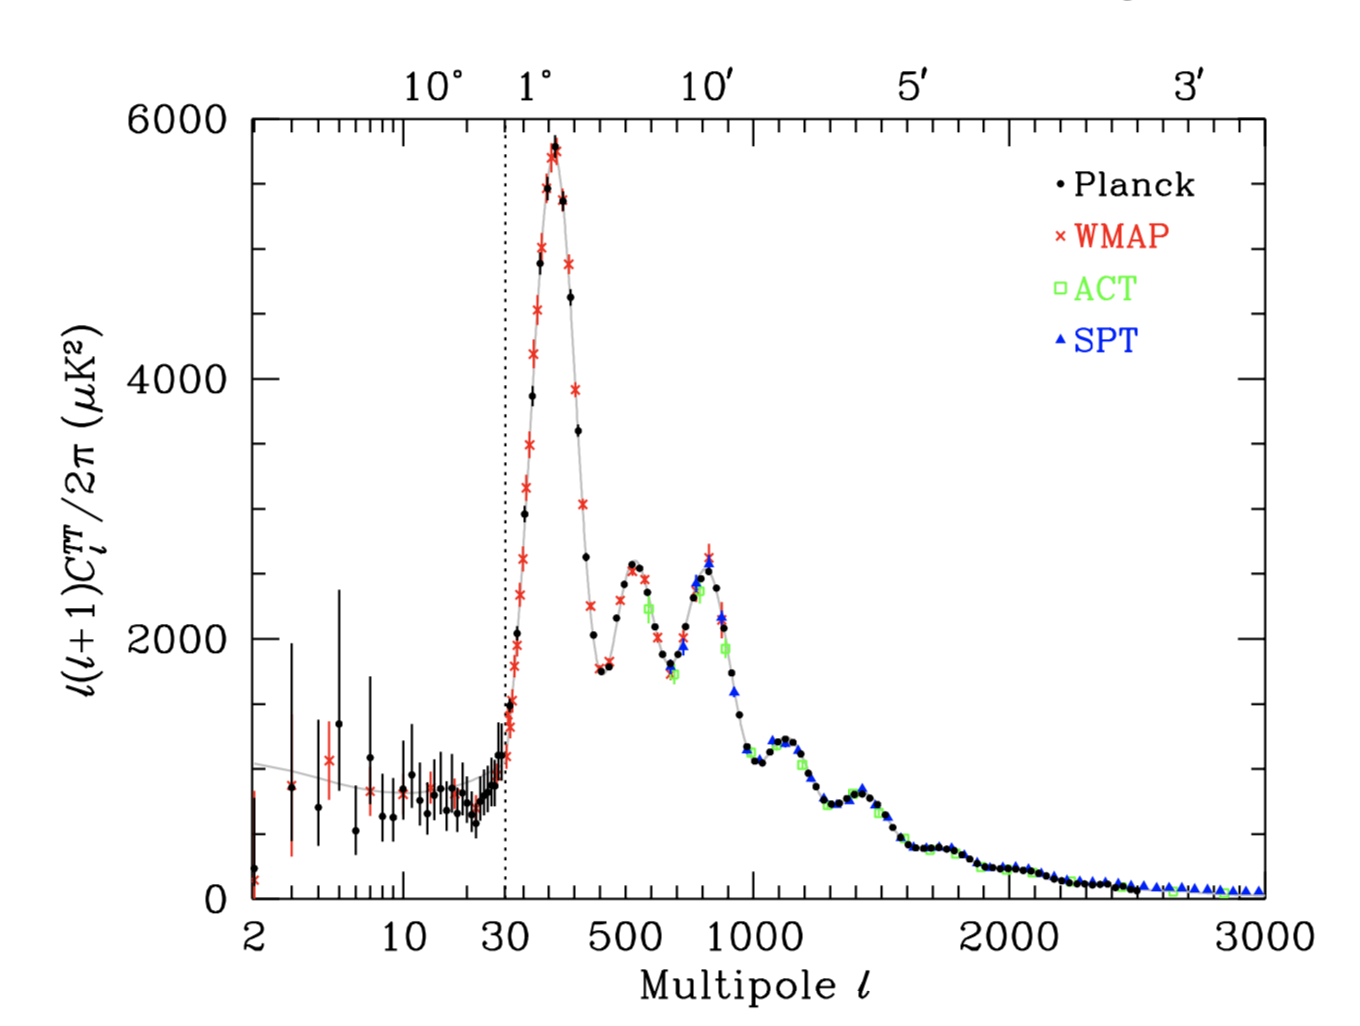
\includegraphics[width=0.8\textwidth]{figs/CMB_multipole}
  \caption{The CMB radiation temperature anisotropy power spectrum as a function of the multipole order,$\ell$, as measured by various experiments~\cite{Agashe:2014kda}. The angular scales that correspond to the multipole orders are listed across the top of the graph. The data points correspond to the experimental measurements and the error bars account for measurement uncertainties. The black curve represents the best global fit of the standard model of cosmology to the Planck data.}
  \label{fig:CMB}
\end{figure}

%In addtion, the numerical simulations  The observation that star ages within galaxies are on the order of 10 to 14 billion years old, and cluster formation is still under way serves to support the cold dark matter (CDM) hypothesis. In this case, DM comprises of rather massive, slow moving, and non-relativistic particles, which would stimulate the clumping of matter into small regions initially, eventually giving rise to larger scale structures. This bottom-up theory of structure formation is further supported by myriad computer simulations consisting of billions of dark matter particles confirming the CDM model yields large structures such as those observed by the Sloan Digital Sky Survey. 

\section{The Standard Model}
\label{sec:SM}

\subsection{Dark matter candidates}
\label{subsec:DMcandidates}

\section{Dark matter detection}
\label{sec:DMsearches}

\subsection{Direct detection}
\label{subsec:DD}

\subsection{Indirect detection}
\label{subsec:ID}

\subsection{Collider searches}
\label{subsec:Collider}


\section{Simplified models of DM: beyond the Standard Model}
\label{sec:BSM}



